%%%%%%%%%%%%%%%%%%%%%%%%%%%%%%%%%%%%%%%%%%%%%%%%%%%%%%%%%%%%%%%%%%%%%%
%% DDIM-LI manuscript -- target: npj Climate and Atmospheric Science %%
%% Built on Springer Nature's official sn-jnl template (sn-nature     %%
%% style option: "Style for submissions to Nature Portfolio          %%
%% journals" -- confirmed correct for npj via web search this        %%
%% session, see WRITING_RULES.md).                                   %%
%%                                                                    %%
%% Per the template's own instruction, this is kept as ONE .tex      %%
%% file (no \input of separate section files) -- Springer Nature's   %%
%% submission systems expect a single manuscript file.                %%
%%                                                                    %%
%% STATUS: DRAFT. Sections marked [PLACEHOLDER] are not yet written  %%
%% -- do not compile-and-submit without replacing every placeholder. %%
%% See manuscript/MANUSCRIPT_PLAN.md and manuscript/citations_ledger.md%%
%% for what's still outstanding.                                     %%
%%%%%%%%%%%%%%%%%%%%%%%%%%%%%%%%%%%%%%%%%%%%%%%%%%%%%%%%%%%%%%%%%%%%%%

\documentclass[pdflatex,sn-nature]{sn-jnl}% Style for submissions to Nature Portfolio journals

\usepackage{graphicx}%
\usepackage{multirow}%
\usepackage{amsmath,amssymb,amsfonts}%
\usepackage{amsthm}%
\usepackage{mathrsfs}%
\usepackage[title]{appendix}%
\usepackage{xcolor}%
\usepackage{textcomp}%
\usepackage{manyfoot}%
\usepackage{booktabs}%
\usepackage{geometry}%

\raggedbottom

\begin{document}

\title[Probabilistic lightning nowcasting over Central Africa]{%
[PLACEHOLDER TITLE -- draft once Results/Discussion are finalized;
avoid overlapping language with Dai et al. 2025's "four-hour
thunderstorm nowcasting" framing, see FINDINGS.md F3b]}

%% [PLACEHOLDER author block -- real names/affiliations/ORCIDs not
%% available from this sandboxed environment]
\author*[1]{\fnm{[First]} \sur{[Author]}}\email{[email]}
\affil*[1]{\orgdiv{[Department]}, \orgname{[Institution]}, \orgaddress{\city{Tel Aviv}, \country{Israel}}}

\abstract{%
[PLACEHOLDER -- not yet drafted, see manuscript/sections/abstract.md
for the planned structure. Draft last, after Results/Discussion are
finalized, per standard practice -- the abstract summarizes the paper,
so writing it first risks having to rewrite it anyway.]
}

\keywords{lightning nowcasting, diffusion model, probabilistic forecasting, satellite remote sensing, Central Africa, deep learning}

\maketitle

\section{Introduction}\label{sec:intro}

[PLACEHOLDER -- not yet drafted. Needs citation verification first
(lightning hazard statistics, Central Africa lightning climatology) --
see manuscript/citations\_ledger.md's "not yet searched" list.
manuscript/sections/introduction.md has the planned outline/flow.
Requires an explicit differentiation paragraph against Dai et al.\
2025 (FINDINGS.md F3b) -- that paper has only been seen via
abstract/search snippets so far, needs a full read before this
paragraph is drafted.]

\section{Results}\label{sec:results}

We developed a probabilistic lightning nowcasting system based on the
elucidated diffusion model (EDM) framework \citep{karras2022edm},
trained on infrared brightness temperature and lightning-imager
observations from the MTG-FCI geostationary instrument over four
regions of Central Africa. The model takes a 6-hour observation history
(36 frames at 10-minute resolution) as context and generates a
probabilistic forecast of lightning occurrence over the following hour
(six 10-minute steps), sampled as an ensemble of 50 physically
plausible realizations per forecast (Fig.~\ref{fig:overview}).

\begin{figure}[t]
\centering
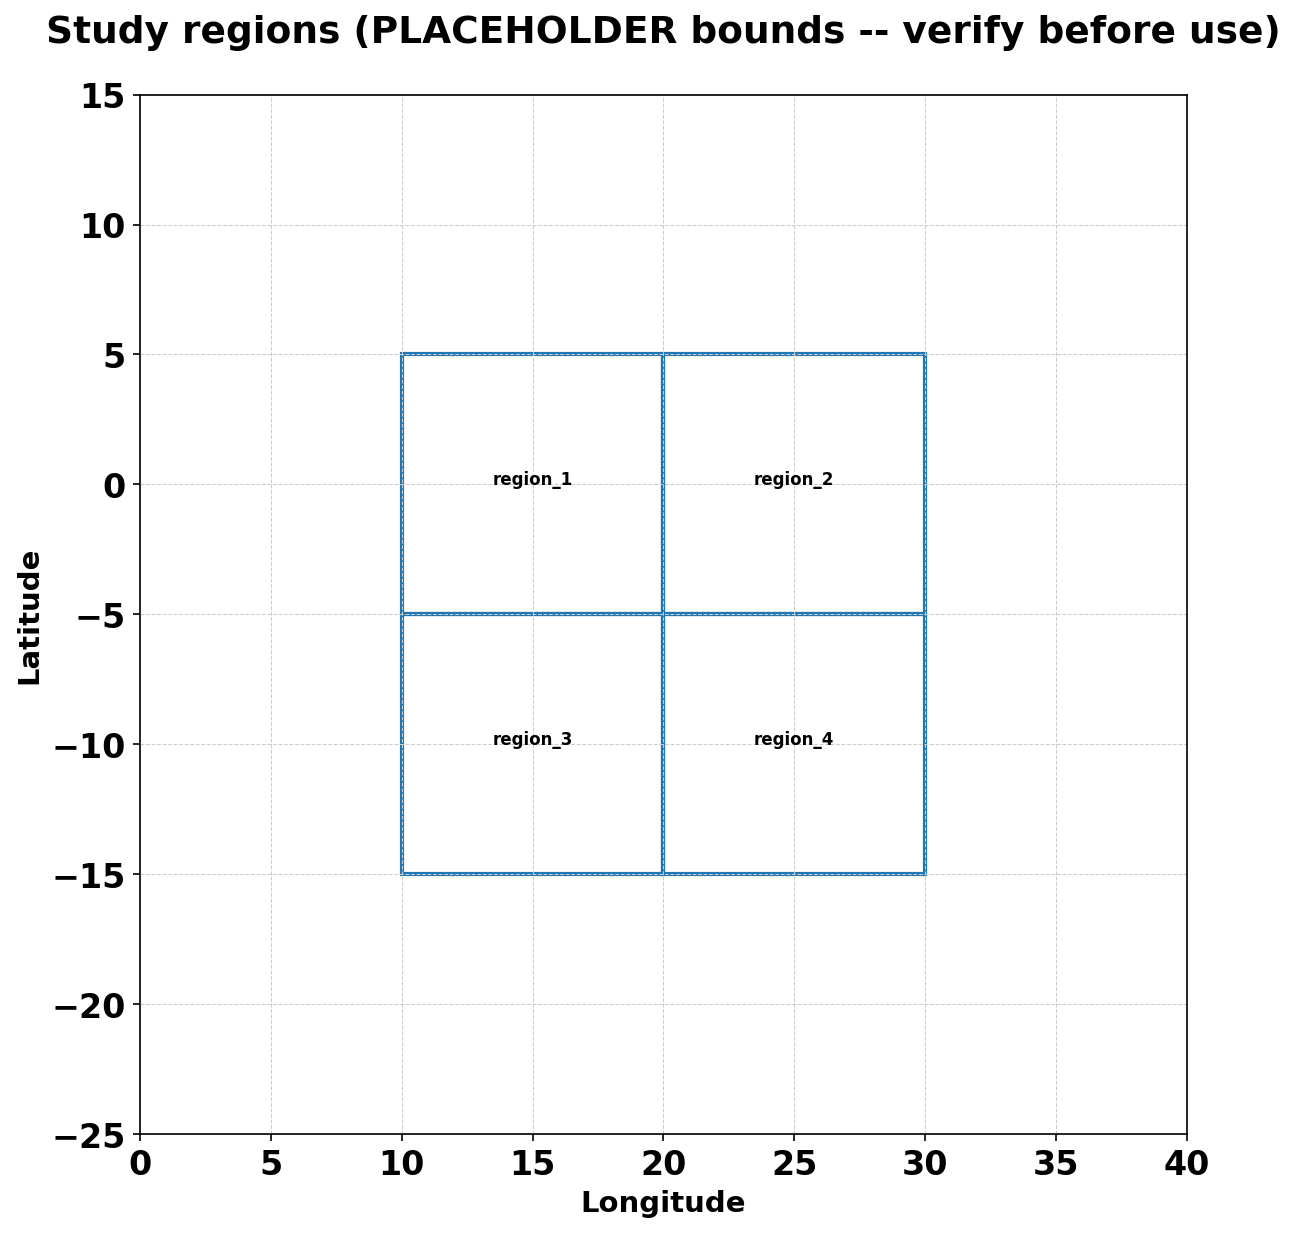
\includegraphics[width=0.85\textwidth]{../figures/fig1_overview.png}
\caption{\textbf{Study overview.} (a) Study region: four test areas
within Central Africa. (b) Model schematic: 6-hour observation context
processed by the EDM diffusion model, sampled as an ensemble of
physically plausible forecast realizations.}
\label{fig:overview}
\end{figure}

\subsection*{The model substantially outperforms physical extrapolation baselines, with an advantage that grows with lead time}

We compared the model's pixel-wise precision-recall AUC (PR-AUC)
against three physically-motivated baselines: persistence, and two
variants of optical-flow extrapolation (pySTEPS-style
semi-Lagrangian advection \citep{pulkkinen2019pysteps}) driven
respectively by the lightning-imager and infrared channels. Across the
six 10-minute lead-time steps tested (+10 to +60 minutes), the model's
PR-AUC ranged from 0.846 to 0.631, compared with 0.783 to 0.391 for
persistence --- the strongest of the three physical baselines at every
lead time except +60 minutes, where the LI-derived optical-flow
baseline narrowly exceeded it (0.392 versus 0.391). The model's margin
over the best available physical baseline grew from 8.1\% at +10
minutes to 61.0\% at +60 minutes (Fig.~\ref{fig:headline}).

Using sequence-level paired bootstrap confidence intervals (1{,}000
resamples, resampling whole test sequences rather than individual
pixels to respect within-scene spatial correlation), every one of these
comparisons was statistically significant (95\% CI excluding zero) at
every lead time tested, with the margin growing monotonically for all
three baselines (persistence: +0.063 to +0.241; LI-derived optical
flow: +0.075 to +0.239; IR-derived optical flow: +0.205 to +0.355;
Fig.~\ref{fig:headline}).

\begin{figure}[t]
\centering
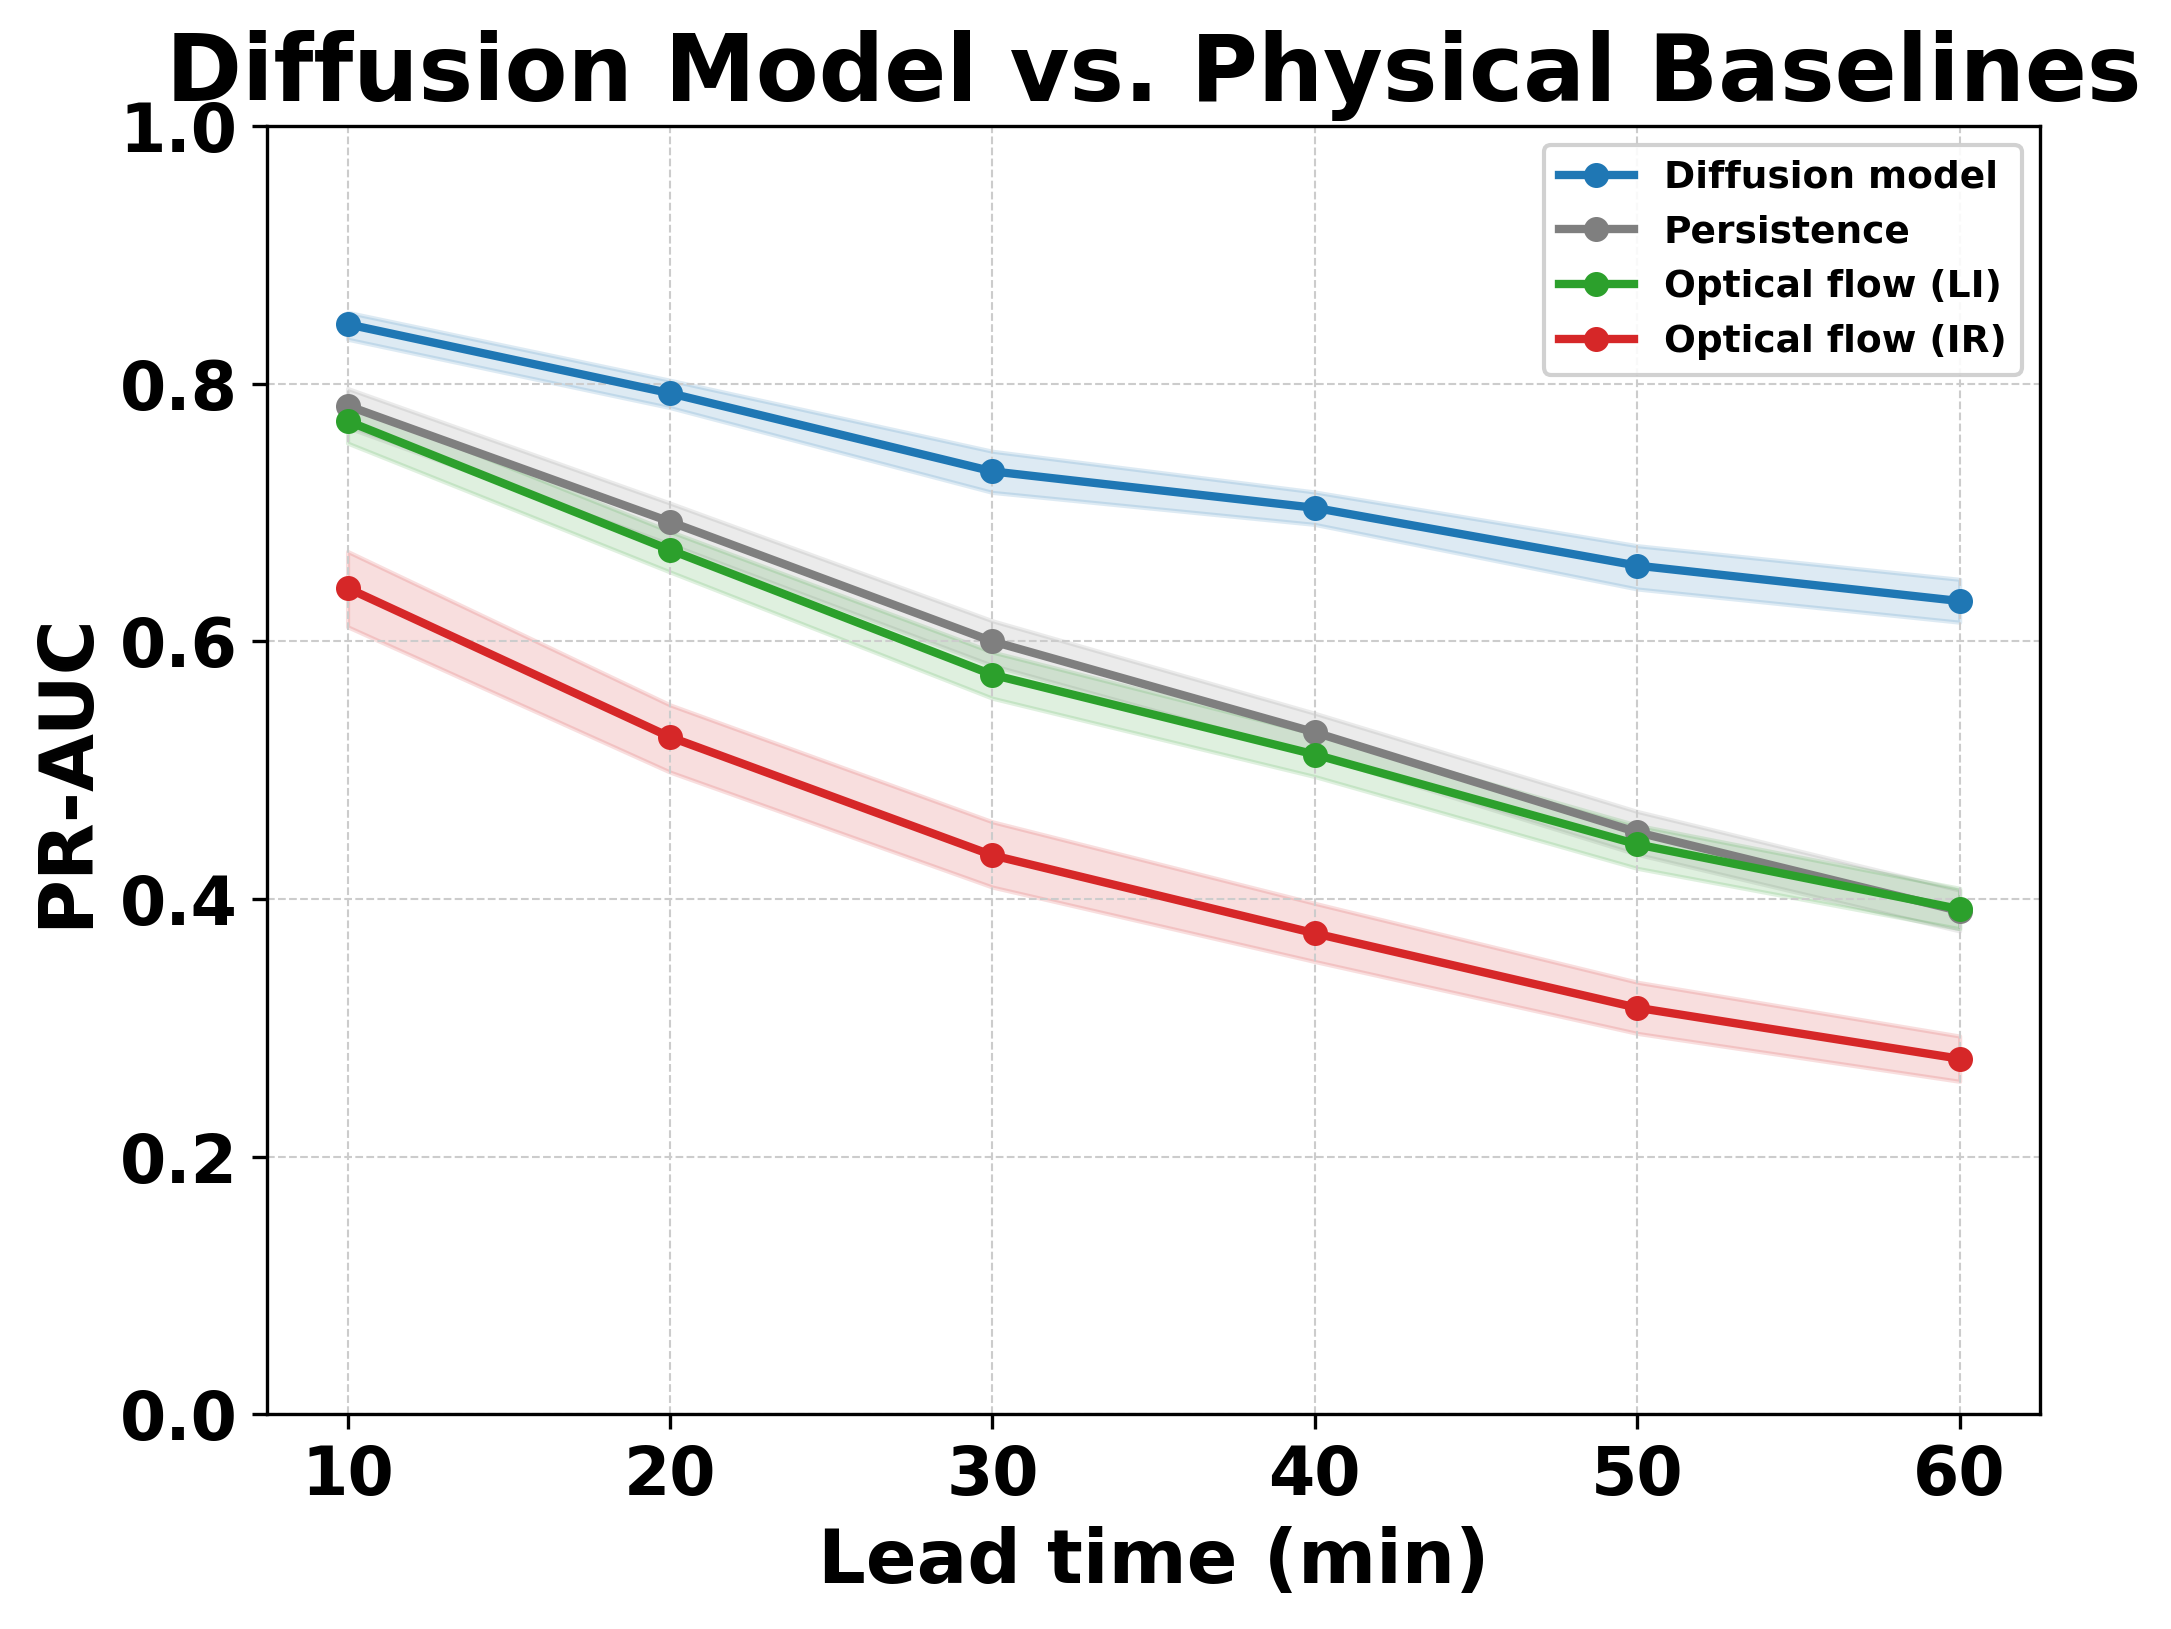
\includegraphics[width=0.85\textwidth]{../figures/fig2_headline_performance.png}
\caption{\textbf{Headline performance.} PR-AUC vs.\ lead time for the
model and the three physical baselines (persistence, LI-derived and
IR-derived optical flow), with 95\% sequence-level paired bootstrap
confidence bands.}
\label{fig:headline}
\end{figure}

\subsection*{Lightning displacement at convective scale is not captured by any coherent motion field}

If residual positional error were explained by a single coherent
motion field --- the entire forecast scene displaced by one
translation vector, as assumed implicitly by any advection-based
extrapolation method --- then scoring each forecast against the
best-possible single global shift of the observed field should recover
most of the skill unlocked by tolerating position error generally.
We tested this directly by comparing exact pixelwise PR-AUC against
(i) the best achievable score under an unconstrained per-scene global
shift and (ii) scores under local neighbourhood tolerance (spatial
pooling at 12, 20, and 28~km radii, with no shift constraint), across
sequences from the test set.

The best global shift recovered only a small fraction of the skill
available under local spatial tolerance, and this fraction did not
increase with lead time. At +10~minutes, allowing the single best
global shift improved PR-AUC from 0.783 to 0.786 --- 7\% of the gain
available from 12~km neighbourhood tolerance alone (0.831). At
+60~minutes, the corresponding improvement was 0.524 to 0.538, or 16\%
of the 12~km-tolerance gain (0.612), and a substantially smaller
fraction of the gain available at 28~km tolerance (0.676;
Fig.~\ref{fig:displacement}). If the model's positional errors were
predominantly a coherent, correctable displacement, the best-shift
curve should approach the neighbourhood-relaxed curves as tolerance
radius increases; instead it remains close to the exact, unrelaxed
score at every lead time tested. This is consistent with positional
error that is spatially heterogeneous at the pixel level rather than a
single global translation, and provides direct, model-independent
evidence for why advection-based extrapolation baselines (persistence,
optical flow) cannot close the gap to the model at these lead times
(cf.\ Fig.~\ref{fig:headline}): there is no single motion field for
them to estimate.

\begin{figure}[t]
\centering
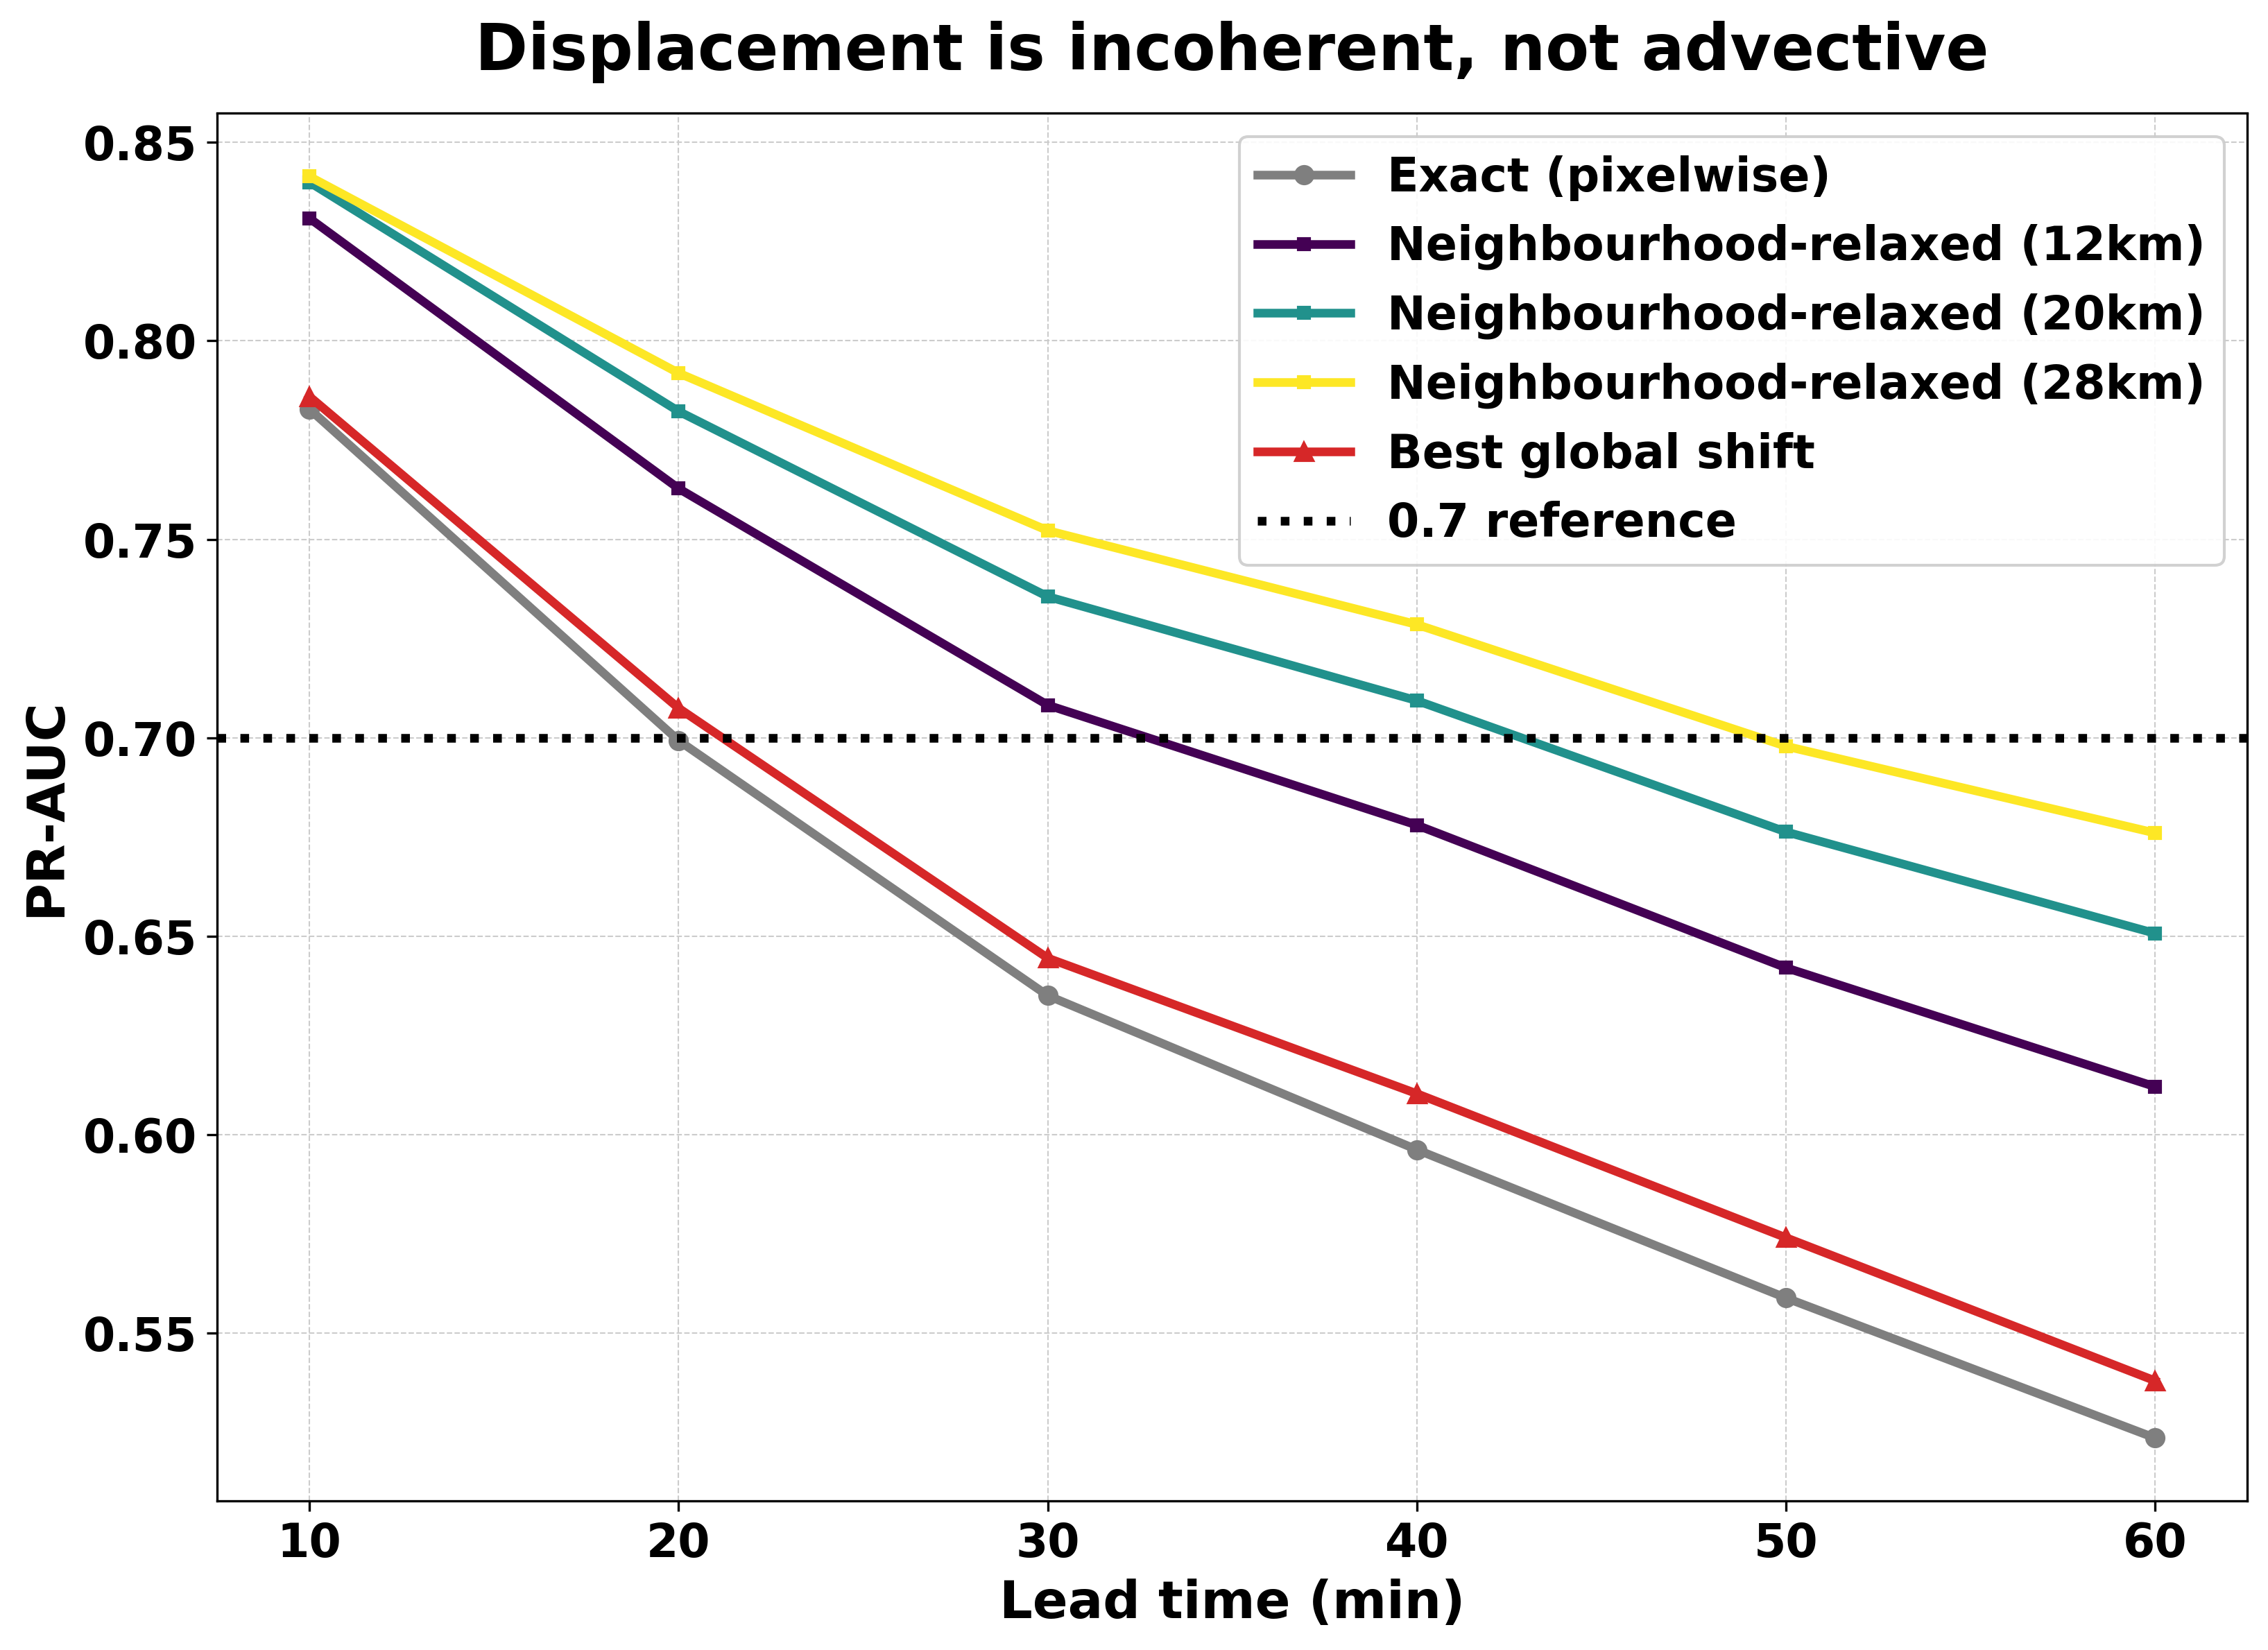
\includegraphics[width=0.8\textwidth]{../figures/fig3_incoherent_displacement.png}
\caption{\textbf{Displacement is incoherent, not advective.} PR-AUC
vs.\ lead time under increasing spatial tolerance: exact pixelwise
scoring, neighbourhood-relaxed scoring at several radii, and the
best-case global-shift upper bound. Convergence of the relaxed and
best-shift curves toward, but not beyond, a common ceiling indicates
positional error is not explained by a single coherent motion field.}
\label{fig:displacement}
\end{figure}

\subsection*{Example forecasts illustrate calibrated ensemble diversity}

[PLACEHOLDER --- checked the actual committed
fig4\_example\_case\_\{low,moderate,high\}\_activity.png files directly
(2026-08-21): all three currently show a real, structured context
frame but a completely blank ground-truth panel and blank ensemble
members. This matches the exact symptom of a bug already found and
fixed in select\_example\_cases.py this session (a double application
of the physical-space transform on the li channel -- see git history)
-- these three files were generated before that fix and need to be
regenerated, not just described from what's currently committed.
Re-run: \texttt{python select\_example\_cases.py --config
configs/evaluate.yaml --checkpoint <path> --output\_dir
manuscript/figures --n\_scan 60 --n\_members 50}, then this subsection
can be drafted from the real, corrected output. Automatic case
selection (ranked by ground-truth activity) may also not be the most
illustrative set -- consider \texttt{--candidate\_indices} once
corrected output can be inspected, per MANUSCRIPT\_PLAN.md's Figure 4
notes.]

\begin{figure}[t]
\centering
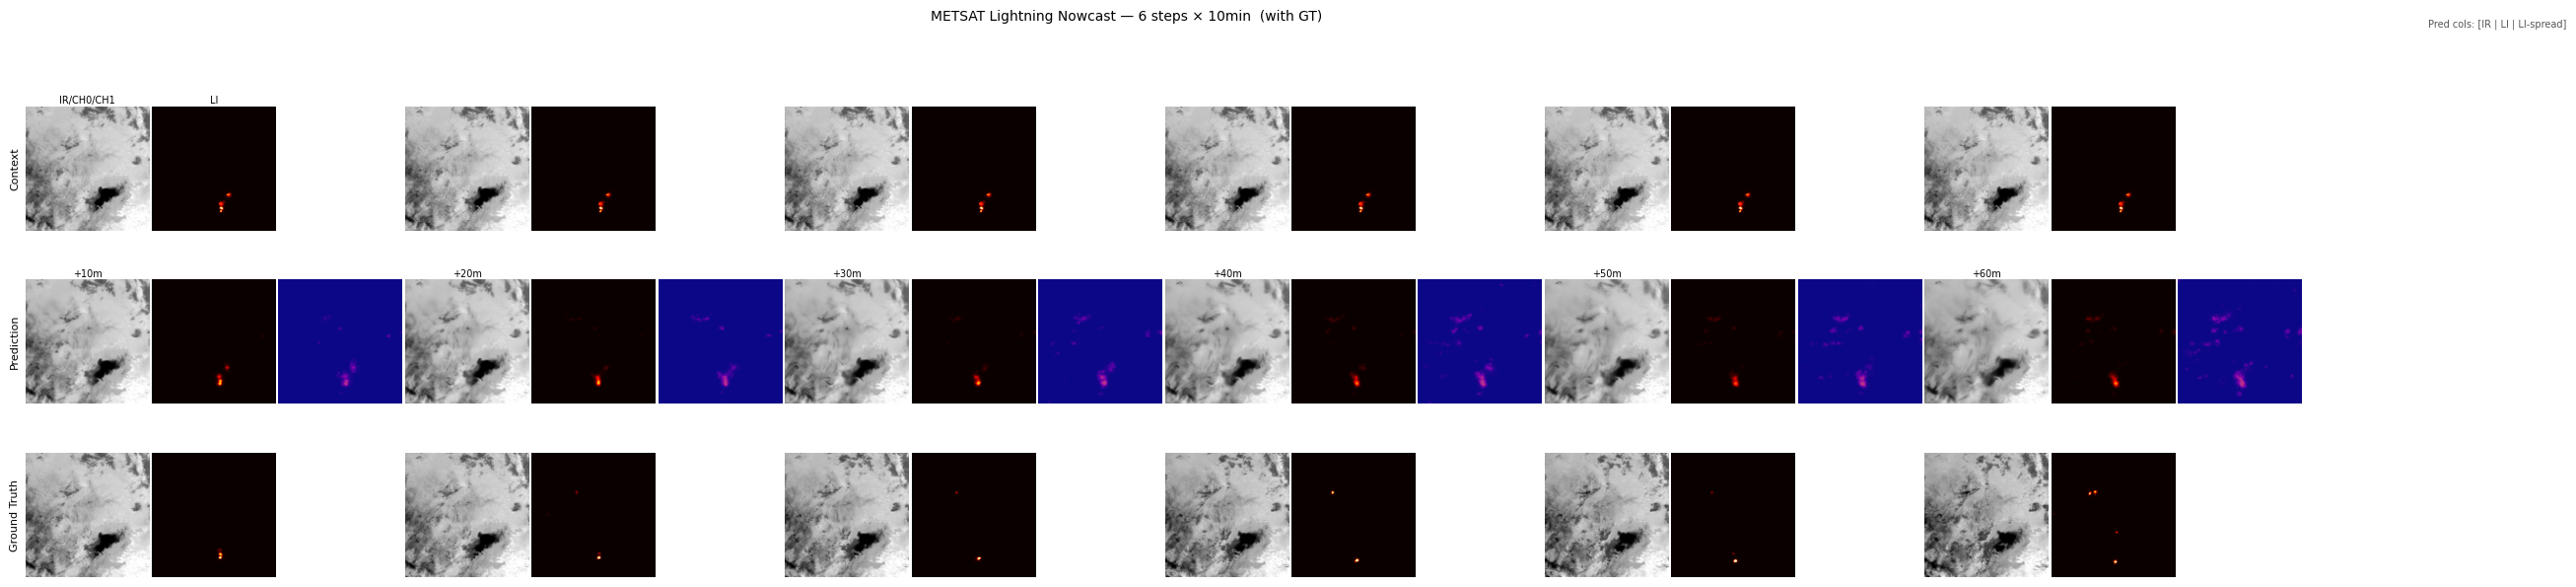
\includegraphics[width=0.85\textwidth]{../figures/fig4_example_case_low_activity.png}\\[4pt]
(a) Low-activity case\\[10pt]
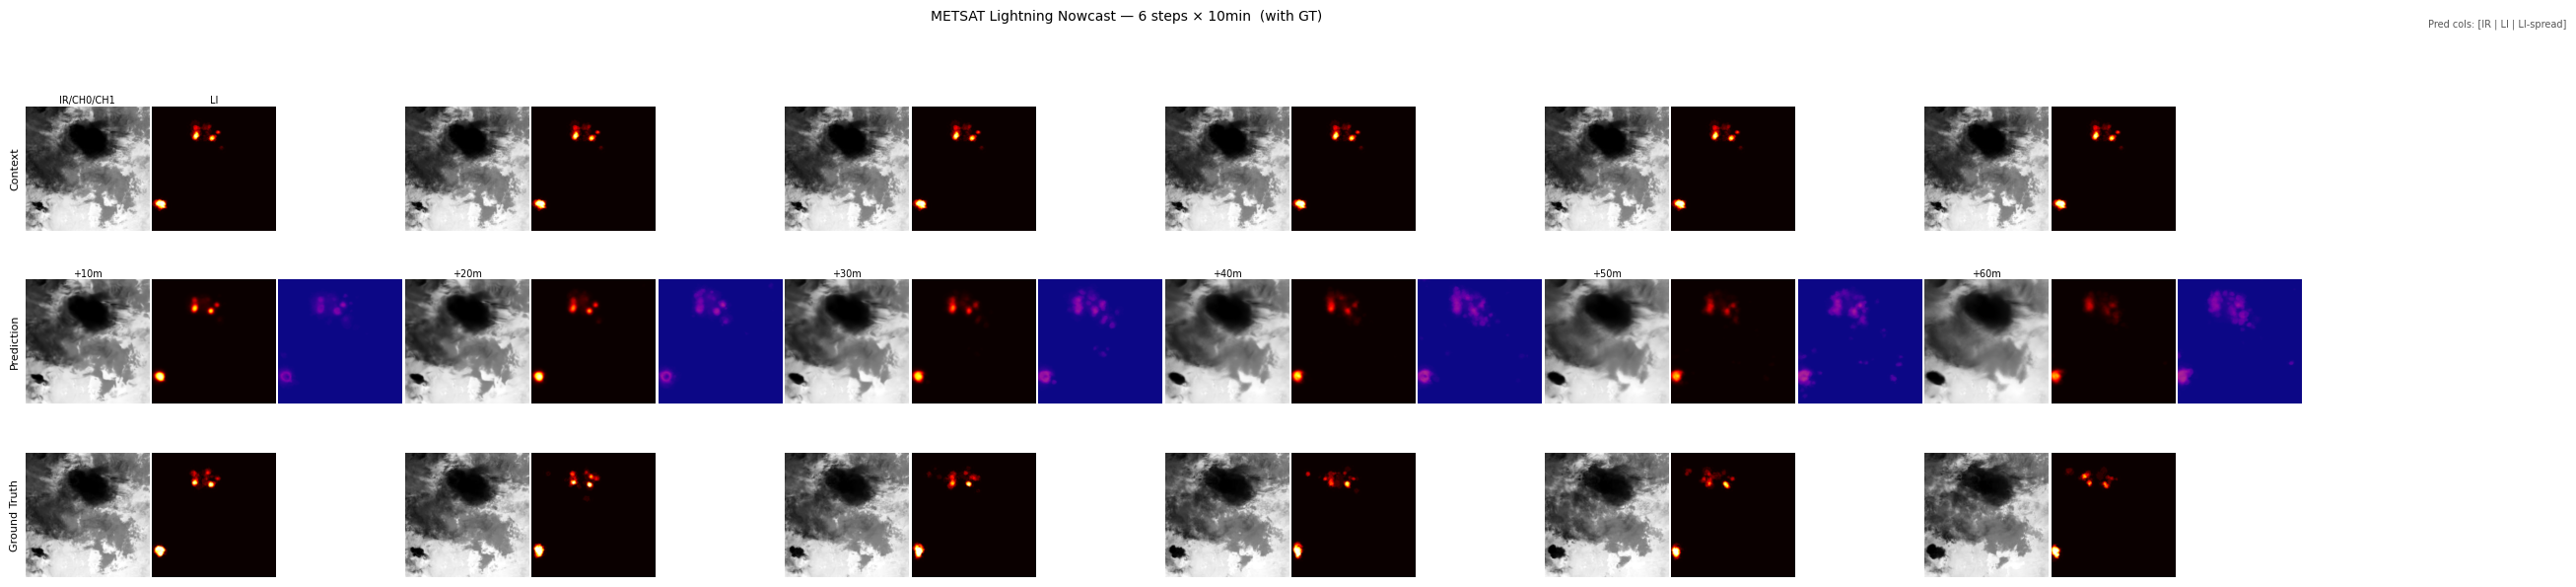
\includegraphics[width=0.85\textwidth]{../figures/fig4_example_case_moderate_activity.png}\\[4pt]
(b) Moderate-activity case\\[10pt]
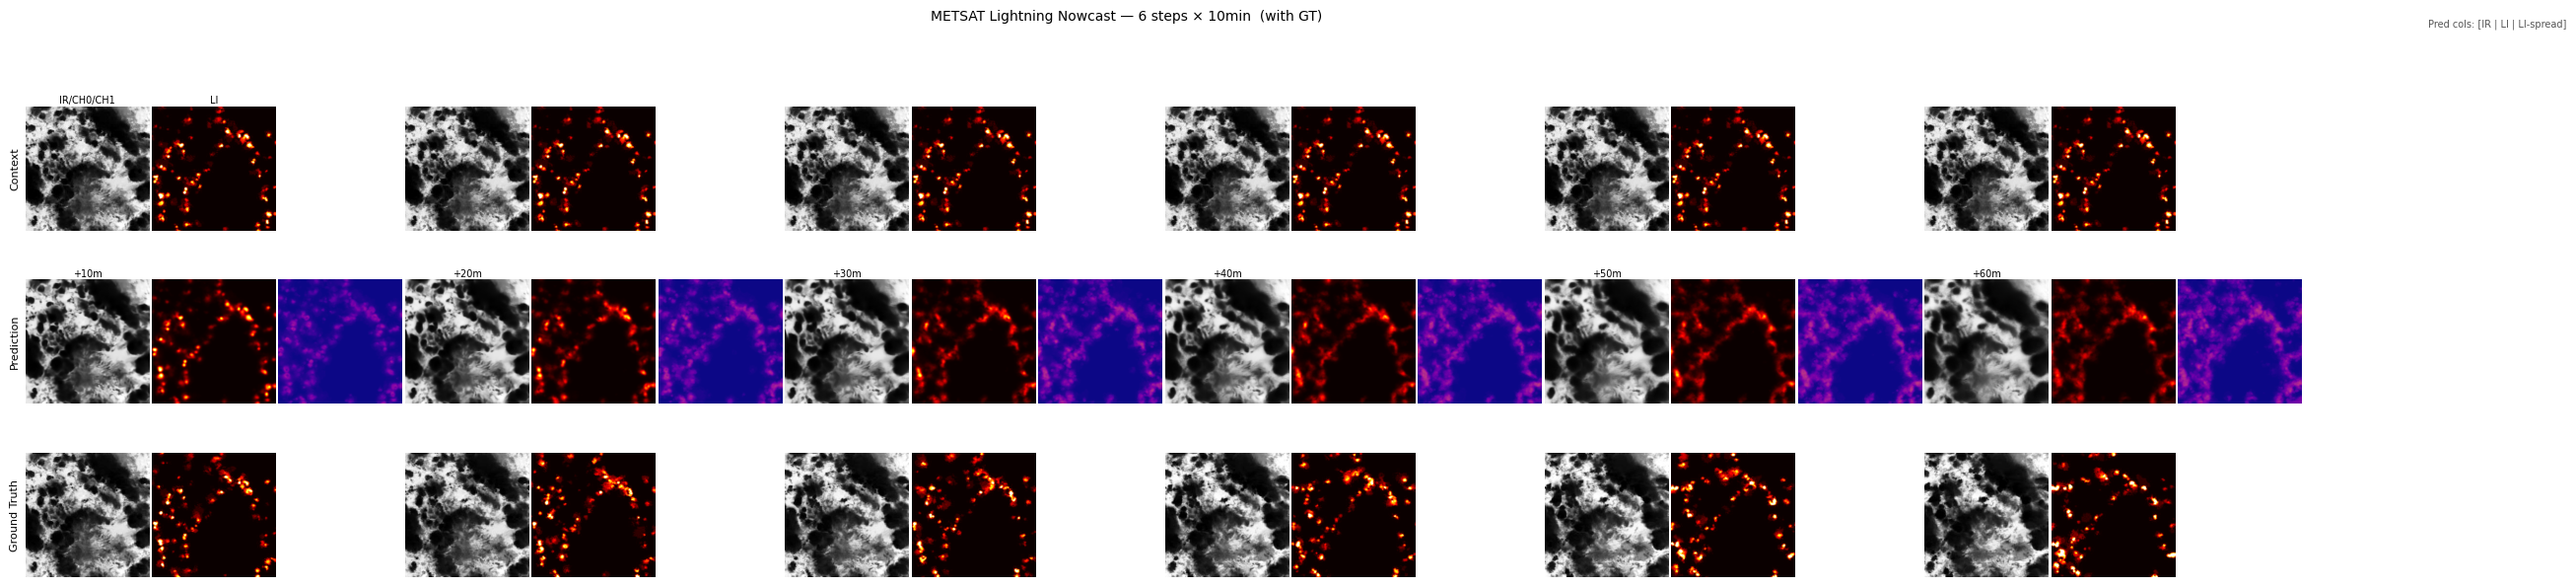
\includegraphics[width=0.85\textwidth]{../figures/fig4_example_case_high_activity.png}\\[4pt]
(c) High-activity case
\caption{\textbf{Example forecasts.} Three representative test
sequences spanning the observed range of lightning activity, each
showing the final observed context frame, ground truth at +60~minutes,
and individual ensemble member samples. [PLACEHOLDER: case selection
here is automatic (ranked by ground-truth activity level), not
necessarily the most illustrative uncertain/multimodal or failure case
-- see select\_example\_cases.py's \texttt{--candidate\_indices} option
and MANUSCRIPT\_PLAN.md's Figure 4 notes for manually curating a better
set once real output has been inspected.]}
\label{fig:examples}
\end{figure}

\subsection*{A directly-optimized deterministic classifier retains a narrow, lead-time-independent pointwise advantage, explained by information access rather than model class}

To assess how the model compares against directly-optimized machine
learning baselines --- not just physical extrapolation --- we trained a
convolutional neural network (CNN) baseline, architecturally and in
training recipe matched to Metzl et al.\ \citep{metzl2025physical}, and
a LightGBM \citep{ke2017lightgbm} baseline using hand-engineered
features, in the methodological spirit of Song et al.\
\citep{song2023lightning}. Both baselines' respective training
objectives (binary cross-entropy for the CNN, logistic loss for
LightGBM) directly match the pointwise verification metric used here,
unlike the diffusion model's own training objective.

The model significantly outperformed LightGBM at every lead time, with
a margin that grew from +0.018 at +10 minutes to +0.185 at +60 minutes
--- the same qualitative shape as the three physical baselines. Against
the CNN baseline, however, the model showed a small but statistically
significant pointwise disadvantage at every lead time (-0.021 to
-0.024), and unlike every other comparison, this margin remained
essentially constant across the full 50-minute range tested rather than
growing (Fig.~\ref{fig:verification}b; see Discussion for
interpretation of this lead-time-independent shape).

This pointwise disadvantage against the CNN baseline was concentrated
at loose probability thresholds and did not persist under spatial
tolerance: at a strict, majority-consensus probability threshold
($p > 0.5$), the model's Fractions Skill Score matched or exceeded the
CNN baseline's at spatial scales beyond approximately 130~km
(Fig.~\ref{fig:verification}a). We further found that this pointwise
gap was substantially, though not entirely, attributable to the
ensemble size used to construct the model's per-pixel probability
estimate: increasing the ensemble from 10 to 50 members closed roughly
60\% of the original PR-AUC gap against the CNN baseline, with a
clearly diminishing-returns pattern (49\% of the gap closed increasing
from 10 to 30 members, a further 21\% of the remainder closed from 30
to 50; Fig.~\ref{fig:verification}b).

\begin{figure}[t]
\centering
\fbox{\begin{minipage}{0.85\textwidth}\centering\vspace{3cm}
\textit{Figure pending --- generate via manuscript/generate\_figures.ipynb\\(fig5a\_fss\_vs\_scale.png not yet generated)}
\vspace{3cm}\end{minipage}}\\[4pt]
(a) FSS vs.\ spatial scale, diffusion model vs.\ CNN baseline\\[10pt]
\fbox{\begin{minipage}{0.55\textwidth}\centering\vspace{2cm}
\textit{Figure pending\\(fig5b\_n\_members\_sensitivity.png not yet generated)}
\vspace{2cm}\end{minipage}}\\[4pt]
(b) Ensemble-size sensitivity
\caption{\textbf{Why baseline comparison needs care.} (a) Fractions
Skill Score vs.\ spatial neighbourhood scale, model vs.\ CNN baseline,
at three probability thresholds -- the model's disadvantage at loose
thresholds does not persist under spatial tolerance, and reverses at
strict thresholds beyond $\sim$130~km. (b) PR-AUC vs.\ lead time at
ensemble sizes of 10, 30, and 50 members, showing the diminishing-
returns pattern underlying the ensemble-size choice used throughout
this study.}
\label{fig:verification}
\end{figure}

\subsection*{The model provides calibrated, genuine forecast uncertainty}

[PLACEHOLDER --- draft once the reliability diagram and CRPS/spread-skill
numbers from Figure~\ref{fig:uncertainty} are finalized against real
(not synthetic) data. Key point to make here: this is the capability
class the CNN/LightGBM baselines structurally cannot be evaluated on,
since they produce a single deterministic output rather than a
sample-based ensemble.]

\begin{figure}[t]
\centering
\fbox{\begin{minipage}{0.85\textwidth}\centering\vspace{3cm}
\textit{Figure pending --- generate via manuscript/generate\_figures.ipynb\\(fig6\_uncertainty\_quantification.png not yet generated)}
\vspace{3cm}\end{minipage}}
\caption{\textbf{Genuine forecast uncertainty.} (a) Reliability diagram,
one line per lead time. (b) Continuous Ranked Probability Score and
spread-skill ratio vs.\ lead time.}
\label{fig:uncertainty}
\end{figure}

\section{Discussion}\label{sec:discussion}

[PLACEHOLDER --- not yet drafted in this file. A substantial existing
draft covering the baseline-verification portion (the F4 story) exists
at manuscript/discussion\_cnn\_baseline\_comparison.md, written before
these LaTeX/citation rules were established --- needs merging in here
and its citations re-verified against citations\_ledger.md before use.
The remaining Discussion content (interpreting the incoherent-
displacement finding, limitations, future work, broader significance)
is outlined but not drafted in manuscript/sections/discussion.md.]

\section{Methods}\label{sec:methods}

\subsection*{Study region and data}

[PLACEHOLDER: MTG-FCI instrument citation not yet verified --- see
citations\_ledger.md "not yet searched" list. Do not finalize this
paragraph until that citation is resolved.] The study region comprises
four test regions within Central Africa (see Fig.~\ref{fig:overview}a
for exact boundaries). Input data are drawn from the MTG-FCI
geostationary satellite instrument at 4~km spatial resolution and
10-minute temporal resolution, using two channels: an infrared window
channel (ir) and a lightning-imager-derived channel (li). The model
takes a 6-hour context window ($T_{in} = 36$ frames) and forecasts a
1-hour horizon ($T_{out} = 6$ frames at 10-minute steps).

\subsection*{Preprocessing}

Both channels are normalized (z-scored) prior to input. The li channel
additionally undergoes a cube-root transform prior to normalization,
chosen because the transform preserves exact zero values --- physically
meaningful for a channel that is either exactly zero (no lightning
activity) or continuously nonzero --- which matters for the
thresholding convention used consistently throughout evaluation
(ground-truth binarization is always performed in physical space, after
inverting both the z-score and the cube-root transform, using a strict
greater-than-zero threshold for the raw physical field and a small
fixed threshold, 5/255, for probability-style outputs derived from
learned models).

\subsection*{Model architecture}

The model follows the elucidated diffusion model (EDM) framework of
Karras et al.\ \citep{karras2022edm}, implemented as a UNet built from
residual blocks, conditioned on the observation context and on lead
time via a shared embedding pathway. [PLACEHOLDER: confirm exact
base\_channels/channel\_mults/num\_res\_blocks/attn\_resolutions values
against the actual training configuration before finalizing --- these
should be pulled directly from configs/default.yaml or the final
checkpoint's saved args, not from memory.]

\subsection*{Training}

The model was trained with distributed data parallelism across two
GPUs, using exponential moving average (EMA) weights for inference,
automatic mixed precision, and a cosine annealing learning rate
schedule, for 790 epochs on a regenerated, quality-controlled version
of the training dataset.

\subsection*{Ensemble size}

Forecasts are generated as an ensemble of sampled realizations from the
diffusion process. We used 50 ensemble members for all final reported
results, a setting chosen via a controlled sensitivity sweep (10, 30,
and 50 members) that showed a clear diminishing-returns pattern:
tripling the ensemble from 10 to 30 members closed roughly half of an
initially large verification-metric gap against a directly-optimized
deterministic baseline, while a further increase to 50 members closed
only a further fifth of the remainder. We attribute the closed portion
of this gap to a finite-sample bias in the empirical, ensemble-derived
probability estimate at loose classification thresholds, confirmed
directly by comparing each model's predicted-positive area fraction
against the true event area fraction at matched thresholds (see
Discussion).

\subsection*{Baselines}

\textbf{Persistence.} The most recent observed lightning field is used
unchanged as the forecast at every lead time.

\textbf{Optical flow.} Two pySTEPS-style \citep{pulkkinen2019pysteps}
semi-Lagrangian extrapolation baselines, driven respectively by
lightning-imager-derived and infrared-derived motion fields.

\textbf{Convolutional neural network (CNN).} A deterministic UNet-style
classifier trained directly on next-frame lightning occurrence via
per-pixel binary cross-entropy, following the general architecture and
training-recipe choices of Metzl et al.\ \citep{metzl2025physical}
(weight decay and learning-rate schedule matched directly to their
reported values). Two departures from their exact protocol were made
deliberately: the CNN baseline shares the diffusion model's own 6-hour
context window and single-model lead-time amortization (rather than
Metzl et al.'s $\sim$30-minute context and separately-trained
per-lead-time models), to hold input information and model structure
constant across our own internal comparisons --- the more rigorous
choice for isolating model architecture as the controlled variable in
this study specifically, even though it diverges from their literal
setup.

\textbf{LightGBM.} A gradient-boosted-tree classifier
\citep{ke2017lightgbm} trained on 18 hand-engineered features derived
from the same ir/li channels (temporal window statistics,
trend/finite-difference features, local spatial neighbourhood
aggregation, and event-recency features), in the methodological spirit
of Song et al.\ \citep{song2023lightning} --- not a literal reproduction
of their protocol, which uses a different input resolution and feature
set (including aerosol and reanalysis inputs not available to this
study). Class imbalance was addressed via LightGBM's native
class-weighting mechanism rather than the manual resampling used for
the CNN baseline, reflecting standard practice for each respective
model class rather than a forced consistency between them.

\subsection*{Evaluation metrics}

Skill was assessed via pixel-wise precision-recall AUC (PR-AUC),
critical success index / probability of detection / false alarm ratio
at multiple probability thresholds, the Fractions Skill Score (FSS)
\citep{roberts2008fss} at multiple spatial neighbourhood scales
(12--260~km), and the Continuous Ranked Probability Score (CRPS) with
its reliability/resolution/uncertainty decomposition
\citep{gneiting2007scoring}, together with reliability diagrams and
spread-skill relationships to assess ensemble calibration directly.

\subsection*{Statistical testing}

All comparisons between the model and each baseline used sequence-level
(not pixel-level) paired bootstrap confidence intervals, resampling
whole test sequences with replacement (1{,}000 resamples) to respect
within-scene spatial correlation in the data. [PLACEHOLDER: decide
whether the bootstrap methodology needs its own citation beyond
standard practice.]

%%===================================================%%
%% All 6 figures are now embedded inline (near their   %%
%% first \ref{}) using the exact filenames              %%
%% manuscript/generate_figures.ipynb and                %%
%% select_example_cases.py produce, under               %%
%% manuscript/figures/. fig5a/fig5b/fig6 don't exist yet %%
%% as real files as of this commit -- \includegraphics   %%
%% will fail to find them until generated for real.      %%
%% Per the template's own instruction, at final          %%
%% SUBMISSION figures should also be attached separately %%
%% as their own files, not only embedded in the .tex --  %%
%% inline embedding here is for draft-review convenience.%%
%%===================================================%%

\backmatter

\section*{Data availability}
[PLACEHOLDER]

\section*{Code availability}
[PLACEHOLDER --- link to the public repository once finalized.]

\section*{Acknowledgements}
[PLACEHOLDER]

\bibliography{../references}

\end{document}
